%%
%% Copyright 2007, 2008, 2009 Elsevier Ltd
%%
%% This file is part of the 'Elsarticle Bundle'.
%% ---------------------------------------------
%%
%% It may be distributed under the conditions of the LaTeX Project Public
%% License, either version 1.2 of this license or (at your option) any
%% later version.  The latest version of this license is in
%%    http://www.latex-project.org/lppl.txt
%% and version 1.2 or later is part of all distributions of LaTeX
%% version 1999/12/01 or later.
%%
%% The list of all files belonging to the 'Elsarticle Bundle' is
%% given in the file `manifest.txt'.
%%

%% Template article for Elsevier's document class `elsarticle'
%% with numbered style bibliographic references
%% SP 2008/03/01
%%
%%
%%
%% $Id: elsarticle-template-num.tex 4 2009-10-24 08:22:58Z rishi $
%%
%%
\documentclass[preprint,12pt,3p]{elsarticle}

%% Use the option review to obtain double line spacing
%% \documentclass[preprint,review,12pt]{elsarticle}

%% Use the options 1p,twocolumn; 3p; 3p,twocolumn; 5p; or 5p,twocolumn
%% for a journal layout:
%% \documentclass[final,1p,times]{elsarticle}
%% \documentclass[final,1p,times,twocolumn]{elsarticle}
%% \documentclass[final,3p,times]{elsarticle}
%% \documentclass[final,3p,times,twocolumn]{elsarticle}
%% \documentclass[final,5p,times]{elsarticle}
%% \documentclass[final,5p,times,twocolumn]{elsarticle}

%% if you use PostScript figures in your article
%% use the graphics package for simple commands
%% \usepackage{graphics}
%% or use the graphicx package for more complicated commands
%% \usepackage{graphicx}
%% or use the epsfig package if you prefer to use the old commands
%% \usepackage{epsfig}

%% The amssymb package provides various useful mathematical symbols
\usepackage{amssymb}
%% The amsthm package provides extended theorem environments
%% \usepackage{amsthm}

%% The lineno packages adds line numbers. Start line numbering with
%% \begin{linenumbers}, end it with \end{linenumbers}. Or switch it on
%% for the whole article with \linenumbers after \end{frontmatter}.
%% \usepackage{lineno}

%% natbib.sty is loaded by default. However, natbib options can be
%% provided with \biboptions{...} command. Following options are
%% valid:

%%   round  -  round parentheses are used (default)
%%   square -  square brackets are used   [option]
%%   curly  -  curly braces are used      {option}
%%   angle  -  angle brackets are used    <option>
%%   semicolon  -  multiple citations separated by semi-colon
%%   colon  - same as semicolon, an earlier confusion
%%   comma  -  separated by comma
%%   numbers-  selects numerical citations
%%   super  -  numerical citations as superscripts
%%   sort   -  sorts multiple citations according to order in ref. list
%%   sort&compress   -  like sort, but also compresses numerical citations
%%   compress - compresses without sorting
%%
%% \biboptions{comma,round}

% \biboptions{}


\journal{Into to AI Class Rutgers}

\begin{document}

\begin{frontmatter}

\title{Assignment 1 for \texttt{Introduction to Artificial Intelligence} class\tnoteref{label0}}


\author[label1,label2]{Henil Patel}


\author[label5]{Kush Patel}
\address[label5]{Rutgers University}

\author[label1,label5]{Ryan Hutton}


\begin{abstract}
This document is Homework 1 for Introduction to Artificial Intelligence class at Rutgers University Spring 2018.
\end{abstract}


\end{frontmatter}

%%
%% Start line numbering here if you want
%%
% \linenumbers

%% main text
\section{Part 1}
\label{sec1}

Understanding the methods [10 points]: Read the chapter in your textbook on uninformed and informed (heuristic) search and then read the project description again. Make sure that you understand A* and the concepts of admissible and consistent h-values.\\

a) Explain in your report why the first move of the agent for the example search problem from Figure 8 is to the east rather than the north given that the agent does not know initially which cells are blocked.\\

\graphicspath{ {images/} }

%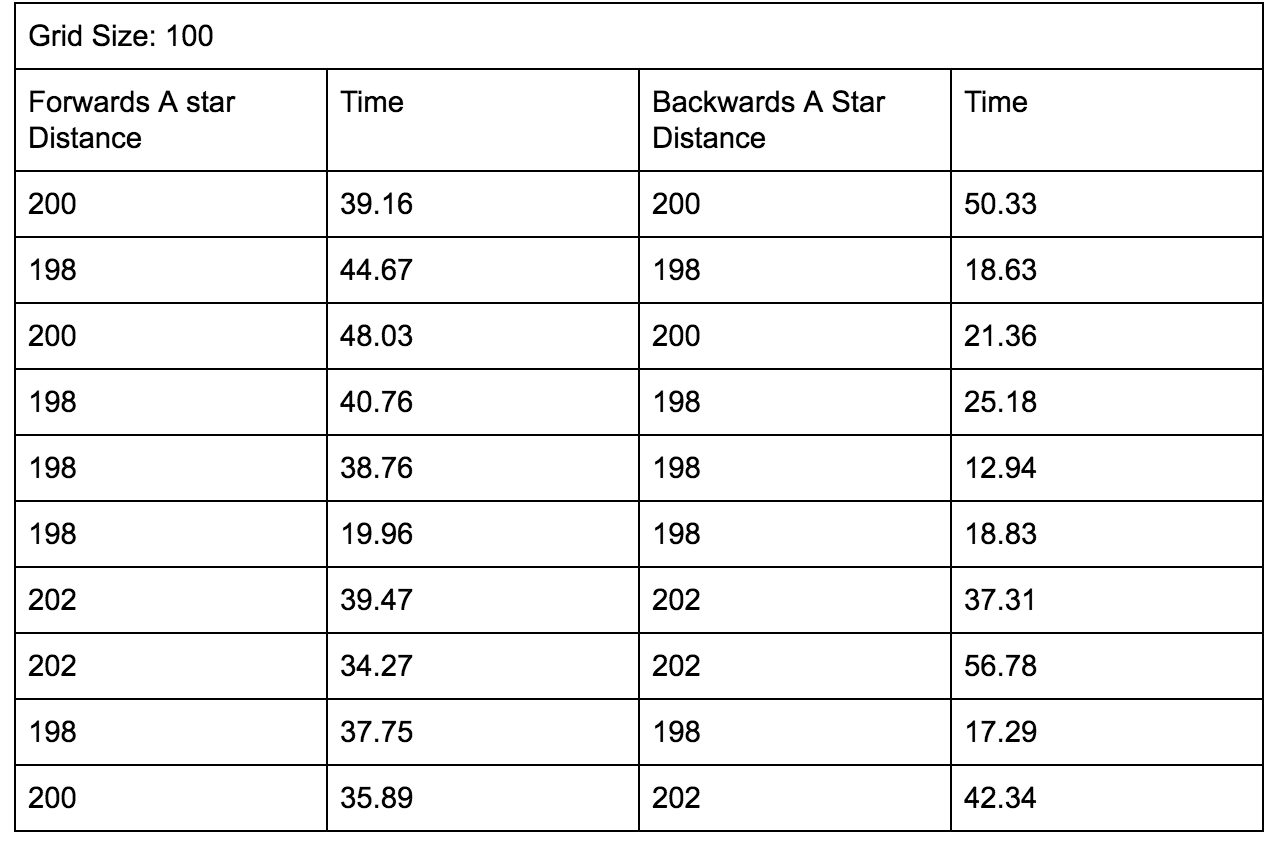
\includegraphics{graph2}
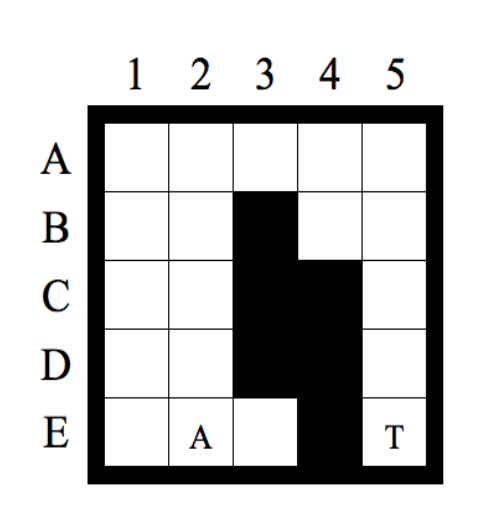
\includegraphics{graph4}

Here, in given algorithm the first move of the agent would be to the east rather than the north because the first step of A* would proceed towards shortest unblocked path. Here, agent is aware that the cell E2 is unblocked, because it would be known in the initial state environment awareness of the agent.


\subsection{Part 1 - B}
\label{subsec1}

Part 1 (b): This project argues that the agent is guaranteed to reach the target if it is not separated from it by blocked cells. Give a convincing argument that the agent infinite grid worlds indeed either reaches the target or discovers that this is impossible in finite time. Prove that the number of moves of the agent until it reaches the target or discovers that this is impossible is bounded from above by the number of unblocked cells squared.\\

Here, agent is in a finite grid world, in the worst case scenario, agent would visit all the unblocked nodes, unless they are not reachable because of being surrounded by blocked nodes. So, when the agent has visited all the nodes, it would have found target and the target must have been added to the open list. Otherwise, target might not have been visited yet, thus open list would be empty. Therefore, algorithm would stop and target will not be found.\\

However, agent does not need to visit all nodes to draw the conclusion about goal not being found. For instance, if the target is blocked by blocked cell around it. In this case, agent would get close to the goal state and rather than going around blocked goal state rather than, finding path far from goal state.\\

Agent will stop after condition $g(goal) = f(goal) \geq f(s) $holds, despite of not visiting all the cells. And agent will determine that it is not possible to find goal in finite time.\\

The number of moves of the agent until it reaches the target or discovers that this is impossible is bounded from above by the number of unblocked cells squared. In the worst case, given a certain number of unblocked nodes n in a certain disposition, algorithm would expand n nodes each time. Therefore, in the worst case, the numbers will be n, expanding n nodes n times, so we have n squared maximum moves.


%% The Appendices part is started with the command \appendix;
%% appendix sections are then done as normal sections

\section{Part 2}
\label{sec2}

The Effects of Ties [15 points]: Repeated Forward A* needs to break ties to decide which cell to expand next if several cells have the same smallest f-value. It can either break ties in favor of cells with smaller g-values or in favor of cells with larger g-values. Implement and compare both versions of Repeated Forward A* with respect to their runtime or, equivalently, number of expanded cells. Explain your observations in detail, that is, explain what you observed and give a reason for the observation.\\ 

[Hint: For the implementation part, priorities can be integers rather than pairs of integers. For example, you can use c X f(s) - g(s) as priorities to break ties in favor of cells with larger g-values, where c is a constant larger than the largest g-value of any generated cell. For the explanation part, consider which cells both versions of Repeated Forward A* expand for the example search problem from Figure 9.]\\

\graphicspath{ {images/} }

%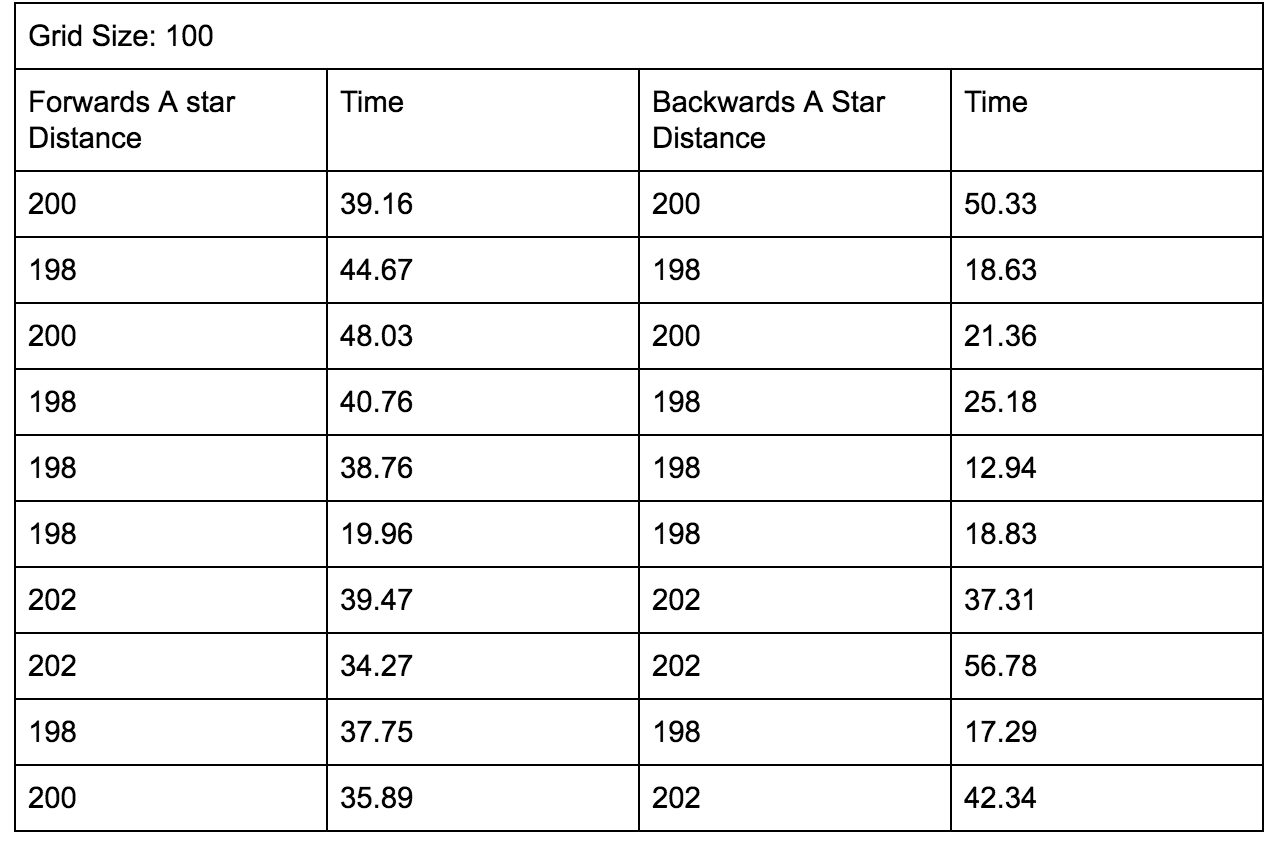
\includegraphics{graph2}
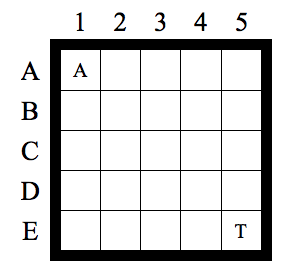
\includegraphics{graph3}

If we compare the two pathfinder algorithms by the number of expanded nodes, we see that the version of Repeated Forward A* breaking ties with higher G-values is faster. A G-value g(s)  is the length of the shortest path from the start state to state s found by the A* search. An h-value (= heuristic) h(s) (which is user-supplied and does not change), which estimates the goal distance of state s, the distance from state s to the goal state. In this case, it is Manhattan Distance. An f-value f(s) := g(s) + h(s), which estimates the distance from the start state via state s to the goal state. Now, in the case of multiple cells that have the same smallest f-value, algorithm can either break ties in favor of cells with smaller g-values or in favor of cells with larger g-values. We see that version where, it favors higher G-Value would be faster because G-value is the length of the shortest path from the start state to state s found. That is, we preferred states closer to the start state than the goal state. Since the goal will be far from the start state, it would be better to reverse the tie-breaking rule, and instead expand states with highest g-cost first.


\section{Part 3}
\label{sec3}

Forward vs. Backward [20 points]: Implement and compare Repeated Forward A* and Repeated Backward A* with respect to their runtime or, equivalently, number of expanded cells. Explain your observations in detail, that is, explain what you observed and give a reason for the observation. Both versions of Repeated A* should break ties among cells with the same f-value in favor of cells with larger g-values and remaining ties in an identical way, for example randomly.\\

We implemented Repeated Forward A* and and Repeated Backward A* with respect to their their runtime in second and considering both algorithms breaking ties at higher G values. If we compare both algorithms by their runtime, we observe that Repeated Backward A* is faster. Here, our mean runtime for Forward A* is 37.872, while mean runtime for Backward A* is 30.099. 

\begin{center}
	\begin{tabular}{||c c c c||} 
		\hline
		Forward A* Distance & Time & Backward A* Distance & Time \\ [0.5ex] 
		\hline\hline
		200 & 39.16 & 200 & 50.33 \\ 
		\hline
		198 & 44.67 & 198 & 18.63 \\
		\hline
		200 & 48.03 & 200 & 21.36 \\
		\hline
		198 &  40.76 & 198 & 25.18 \\
		\hline
		 198 &  38.76 &  198 & 12.94 \\ [1ex] 
		\hline
		\hline
		198 &  19.96 &  198 & 18.83 \\ [1ex] 
		\hline
		\hline
		202 &  39.47 &  202 & 37.31 \\ [1ex] 
		\hline
		\hline
		202 &  34.27 &  202 & 56.78 \\ [1ex] 
		\hline
		\hline
		198 &  37.75 &  198 & 17.29 \\ [1ex] 
		\hline
		\hline
		200 &  35.89 &  200 & 42.34\\ [1ex] 
		\hline
		
		
	\end{tabular}
\end{center}


\graphicspath{ {images/} }

%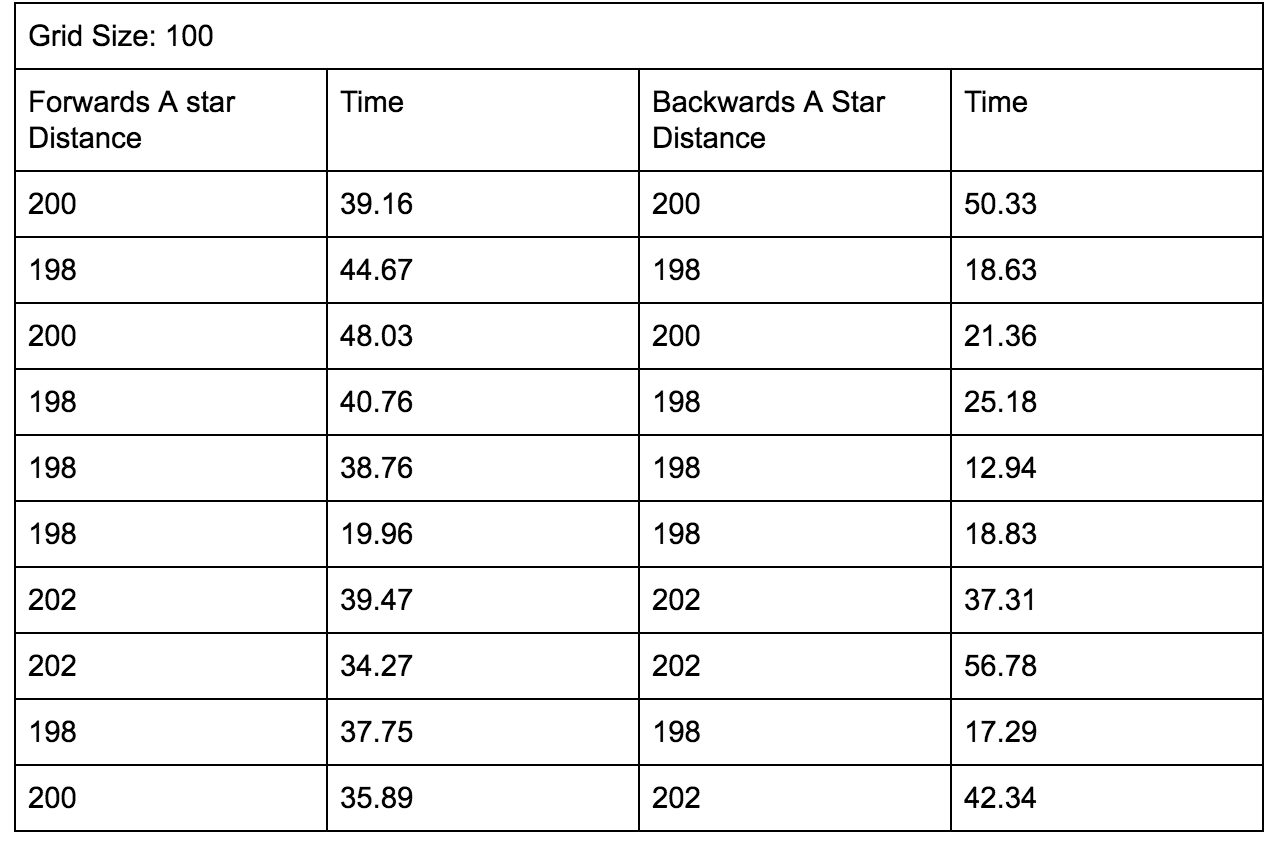
\includegraphics{graph2}
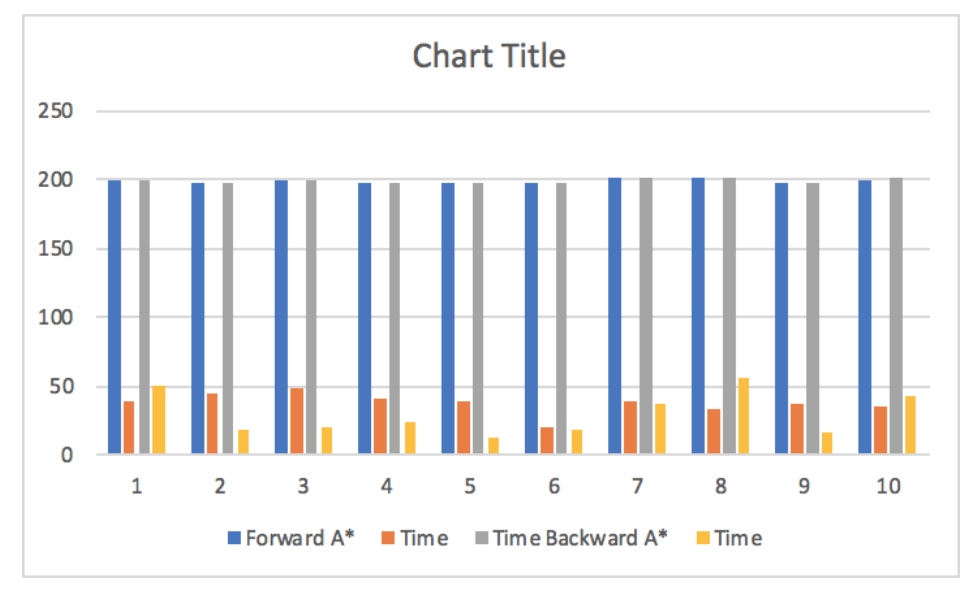
\includegraphics{graph1}

\section{Part 4.1}
\label{sec4}

Heuristics in the Adaptive A* [20 points]: The project argues that “the Manhattan distances are consistent in grid worlds in which the agent can move only in the four main compass directions.” Prove that this is indeed the case.\\ 

Manhattan distances are consistent because they are computed by summing up the shortest possible vertical and horizontal distances. Manhattan distances between two points will always be the same for any horizontal and vertical steps. In our case, agent can not move in diagonal fashion, it only moves in either vertical or horizontal fashion. Thus, this heuristic can never overestimate the cost of reaching the target. 

\subsection{Part 4.2}
\label{subsec4}

Furthermore, it is argued that “The h-values h new(s) ... are not only admissible but also consistent.” Prove that Adaptive A* leaves initially consistent h-values consistent even if action costs can increase.\\

Here, we will prove this considering a grid world where agent could only move in four directions.\\

Consider, H-values are consistent. h(s) follows Manhattan Heuristics and \begin{math} h new(s)  :=  g(goal) - g(s) \end{math} . Also, cost of going from n to $\'{n} $ will be $ c(n,a,\'{n}) $ will be one.\\

Consider, triangle inequality 
\begin{equation} 
h(n)  \leq h(\'{n}) + c(n,a,\'{n})
\end{equation}

The fact that this inequality holds for h(s) tells us that those h-values are consistent.\\

Now, prove that \begin{math}h new (n)  \leq h new(\'{n}) + c(n,a,\'{n})\end{math}.

First, we substitute 
\begin{equation}
h new(n)  :=  g(goal) - g(n) 
\end{equation}

\begin{equation}
h new(\'{n}) = g(goal) - g(\'{n})
\end{equation}

We get \begin{math} g(goal) - g(n) \leq g(goal) - g(\'{n}) + c(n,a,\'{n})$\end{math}\\

Eliminate g(goal) from both sides,
\begin{equation}
g(n) \geq g(\'{n}) + c(n,a,\'{n})
\end{equation}
Here, if the agent can move only in the four main compass directions this equation is always true. Here, c(n,a,\'{n}) is one. If g(\'{n}) is smaller than g(n), then subtracting one from it will make it even smaller. Also, g(\'{n}) is greater than g(n), then subtracting one from it will make them equal. Therefore the triangle inequality is satisfied and the h new (s) values are consistent.\\

H-values h new (n) remain consistent even if action costs can increase. \\
Now, we consider again the triangle inequality: $ h new (n)  \leq h new (\'{n}) + c(n, a, \'{n})$. Let’s assume that there is an action cost increase, where c: action cost before increase $ \'{c}: $ action cost after increase. \\

Thus: $hnew (n) \leq h new (\'{n}) + c(n, a, \'{n}) \leq h new (\'{n}) + \'{c}(n, a, \'{n}).
$
\\
Therefore the heuristic remains consistent.

\section{Part 5}
\label{sec5}
Part 5 - Heuristics in the Adaptive A* [15 points]: Implement and compare Repeated Forward A* and Adaptive A*
with respect to their runtime. Explain your observations in detail, that is, explain what you observed and give a reason for
the observation. Both search algorithms should break ties among cells with the same f-value in favor of cells with larger
g-values and remaining ties in an identical way, for example randomly.\\

Assume that we are running several A* searches with consistent heuristics in the same state space and with the same goal states but possibly different start states. Adaptive A* would always be better than Repeated Forward A*. In Adaptive A* the idea is to make the heuristics more informed after each A* search in order to speed up future A* searches. Adaptive A* uses informed h-values to focus its searches. The initial h-values are provided by the user and must be consistent for the initial action costs. Adaptive A* updates its h-values after each search to make them more informed and focus its searches even better. An iteration of Adaptive A* proceeds as follows: It first updates the action costs, if necessary, to reflect any increases in action costs. It then picks a start state and runs a forward A* search to find a cost-minimal path from the start state to any state in the given set of goal states. Assume that the search determined that the cost of the cost-minimal path is g*. The h-values remain consistent and Adaptive A* thus continues to find cost-minimal paths over time without having to re-expand states during the same search.[Koenig and Likhachev]




\section{Part 6}
\label{sec6}

Memory Issues [10 points]: You performed all experiments in grid worlds of size 101 × 101 but some real-time computer games use maps whose number of cells is up to two orders of magnitude larger than that. It is then especially important to limit the amount of information that is stored per cell. For example, the tree-pointers can be implemented with only two bits per cell. Suggest additional ways to reduce the memory consumption of your implementations further. Then, calculate the amount of memory that they need to operate on grid worlds of size 1001 X 1001 and the largest grid world that they can operate on within a memory limit of 4 M Bytes.\\

Some additional ways of reducing memory consumption of our implementation is to not use cell objects to hold information.\\

We use cells objects to hold the g value, h value, f value, row number, column number, and In addition, we should avoid storing the G-scores for every single nodes, instead only for cells that have been expanded.\\

In addition, cells use large amount of memory. To improve on that, we could use tuples and basic arrays to store information.\\

In addition, we could use reduce number of integers needed for storing information. For example, we could combine cell state and seen variables.\\ 

Also, we could turn previous into pointer instead of list, which takes less memory. By saving less variables, and generating the values dynamically could also save memory space. For example, h values could be generated as we move instead of when the grid is generated.\\

Calculating the amount of memory that they need to operate on grid worlds of size 1001 X 1001 and the largest grid world that they can operate on within a memory limit of 4 M Bytes.\\

Based on python 3.6, Size of integer is 24 bytes.\\

Size of the list with 2 integers is 104 bytes.\\

Each cell contains 7 integers and 1 list with 2 integers.\\

Total size for Cell = (7 X 24) + 104 = 272\\

Number of cells in a 101x101 grid = 101 X 101 = 10201\\

Total memory for 101 x 101 grid = 10201 X 272 = 2,774,672 bytes = 2.775 megabytes\\

Number of cells in 1001x1001 grid = 1001 X 1001 = 1,002,001\\

Total memory for 1001x1001 grid = 1,002,001 X 272 = 272,544,272 bytes =
272.544 megabytes\\

Amount of cells that can fit on 4 megabytes = 4 / 0.000272 = 14,705 cells Grid\\
size = sqrt(14,705) = 121\\

Max size of grid in 4MB = 121x121\\

We could obtain 121 X 121 nodes.\\


\section{References}
\label{sec7}
Koenig and Likhachev, Adaptive A* [Poster Abstract], Proceedings of the International Joint Conference on Autonomous Agents and Multiagent Systems (AAMAS), 1311-1312, 2005

%% References
%%
%% Following citation commands can be used in the body text:
%% Usage of \cite is as follows:
%%   \cite{key}         ==>>  [#]
%%   \cite[chap. 2]{key} ==>> [#, chap. 2]
%%

%% References with bibTeX database:

%\bibliographystyle{elsarticle-num}
% \bibliographystyle{elsarticle-harv}
% \bibliographystyle{elsarticle-num-names}
% \bibliographystyle{model1a-num-names}
% \bibliographystyle{model1b-num-names}
% \bibliographystyle{model1c-num-names}
% \bibliographystyle{model1-num-names}
% \bibliographystyle{model2-names}
% \bibliographystyle{model3a-num-names}
% \bibliographystyle{model3-num-names}
% \bibliographystyle{model4-names}
% \bibliographystyle{model5-names}
% \bibliographystyle{model6-num-names}

%\bibliography{sample}


\end{document}

%%
%% End of file `elsarticle-template-num.tex'.
